\chapter{Scattering Model}
A system of three idenical bosons with $J=0$ and masses $m = m( \prescript{87}{}{\mathrm{Rb}})$ has been considered in this work. We have assumed that the interactions $V(\rho,\theta,\psi)$ can be written as a sum of pairwise two-body potentials   

\begin{equation}\label{eq:potential_sum}
V(\rho,\theta,\psi) = v(r_{12}) + v(r_{23}) + v(r_{31}).
\end{equation} 

Since, the general feature of the Efimov effect is that it is insensitive to the details of the interatomic interaction and that it, to a good approximation, only depends on the scattering length and the interaction range it allows for the use of model potentials, where the scattering length and the number of two-body bound states can be controlled. The two-body potential used here is  

\begin{equation}\label{eq:two_b_potential}
v(r) = d\cosh^{-2}{(r/r_0)},
\end{equation}
where $d$ controls the depth and $r_0$ the range of the potential.
This potential is particularly usefull since the eigenfuctions and energies are known analytically \cite{Landau1965Quantum}. The scattering length can be calculated at different $d$ numerically as described in \cref{sec:zero_energy_scat}, or it can be calculated exactly through 

\begin{equation}
a = \lim_{k \to 0} \frac{1}{ik} \frac{S(k)-1}{S(k)+1}
\end{equation}
in which $S(k)$ is the scattering  using 

\begin{equation}
2^{\varepsilon} \frac{\,_2F_1(-s, s+1, 1-\varepsilon;\frac{1}{2})}{\,_2F_1(\varepsilon-s, \varepsilon + s+1, 1+\varepsilon;\frac{1}{2})}
\end{equation}
where 

The scattering length can  

By changing the interaction strength, the potential can be tuned to support a different number of two-body bound states.   

\begin{figure*}[b!]
	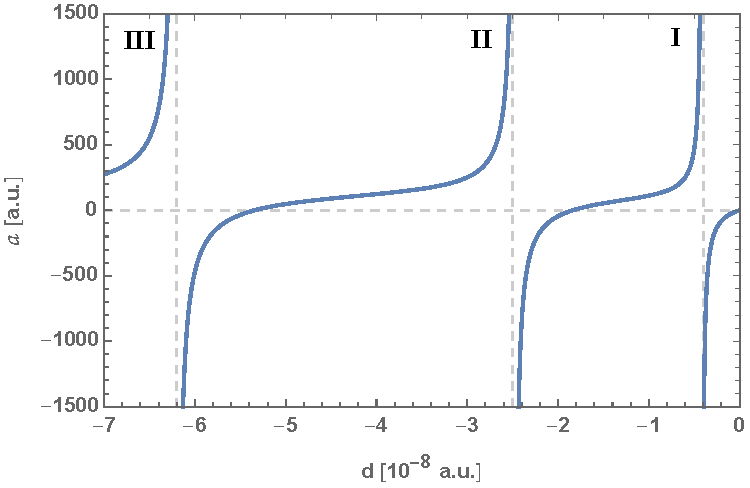
\includegraphics[width=\linewidth]{scatteringlength.pdf}
	\caption{The two-body scattering length as a function of the potential depth $d$. Three poles can be recognized in the figure, labelled $\mathrm{I},\mathrm{II},\mathrm{III}$. At each pole a new two-body bound state is formed. The first bound state is formed as $a$ passes through $\mathrm{I}$, followed by a second a two-body bound state is formed. At each pole a new two-body bound state is formed, so when $\abs{d}$ is increased so that $a$ passes through $\mathrm{II}$ a second two-body bound state is formed, while a third state is formed as $a$ passes through $\mathrm{III}$.}
	\label{fig:res_1}
\end{figure*}